\section{图表类型推荐系统评估}

在完成数据集构建、混合检索方法设计与系统原型实现后，需要进一步检验本文方法是否能够在推荐效果和用户使用体验两个层面支撑自然语言驱动的图表类型推荐任务。单纯观察系统是否能够返回候选图表并不足以说明方法有效，因为推荐系统既需要在算法层面覆盖正确图表类型，也需要在交互层面帮助用户理解、选择和修改推荐结果。因此，本章围绕“推荐是否准确”和“系统是否有用”两个问题展开评估。

本章评估由消融实验和用户研究两部分组成。消融实验主要考察不同数据集、不同文本表示和不同检索策略对推荐结果的影响，用于分析第三章提出的 ChartRWC 数据集以及第四章提出的混合检索流程是否具有实际贡献。用户研究则从真实使用场景出发，观察参与者在系统辅助下完成图表类型选择和图表编辑的过程，并结合问卷结果分析系统界面与推荐结果的可用性。通过两类评估相互补充，本文能够同时从定量指标和用户反馈两个角度说明系统的有效性与局限。

\subsection{消融实验}

本文设计并实施了两个消融实验，用于验证图表描述质量和训练数据来源对检索推荐效果的影响。实验对象包括第四章提出的稀疏检索和稠密检索两类方法。稀疏检索实验关注文本预处理与图表描述语义质量对关键词匹配的影响，稠密检索实验关注多模态编码模型在不同数据集上训练后能否迁移到另一数据分布。两组实验共同回答一个问题：第三章构建的 ChartRWC 是否比原始 ChartGen 更适合作为自然语言图表推荐任务的数据基础。

实验采用交叉数据集设置。本文分别将 ChartGen 和 ChartRWC 作为候选库构建检索索引或训练表示模型，并在同一数据集和另一数据集上进行测试。这里的“训练集”并不只表示监督学习中的参数训练数据，在稀疏检索中也表示用于建立倒排索引和候选图表库的数据集合；“测试集”表示提供查询文本和真实图表类型标签的数据集合。通过这种设置，实验能够同时观察两种情况：模型或索引在同源数据上的表现，以及面对另一种文本风格和图表分布时的泛化能力。

评价指标采用 Top 1 和 Top 5 准确率。对于每一条测试样本，系统根据输入文本返回一个按相关性排序的候选图表列表，并将候选图表的类型与该测试样本的真实图表类型进行比较。若排名第1的候选图表类型与真实类型一致，则该样本计入 Top 1 命中；若排名前5的候选图表中至少有一个与真实类型一致，则该样本计入 Top 5 命中。对某一图表类型而言，Top 1 或 Top 5 数值等于该类型测试样本中命中样本数占总测试样本数的比例。Top 1 反映系统首位推荐是否准确，Top 5 反映系统是否能在有限候选范围内覆盖正确图表类型。消融实验结果如表\ref{tab:gen2rwc} 和表\ref{tab:rwc2gen} 所示。

\subsubsection{图表描述在稀疏检索中的影响}

稀疏检索实验使用第四章中表现最优的策略3进行词语过滤，即同时剔除实体、停用词、助动词、介词、虚词和标点符号。该设置在固定文本预处理方式的前提下，考察 ChartGen 和 ChartRWC 的图表描述本身是否会影响检索能力。实验中，系统将训练集中的图表描述构建为倒排索引，并使用测试集中的文本描述作为查询。每次查询返回排序后的候选图表，随后根据候选图表类型是否与测试样本真实类型一致计算 Top 1 和 Top 5。

表\ref{tab:gen2rwc} 的列结构可以分为两组。第2列至第5列表示以 ChartGen 作为候选库构建索引时的结果，其中第2、3列是在 ChartGen 自身上测试，第4、5列是在 ChartRWC 上测试；第6列至第9列表示以 ChartRWC 作为候选库构建索引时的结果，其中第6、7列是在 ChartRWC 自身上测试，第8、9列是在 ChartGen 上测试。这样的排列可以直接比较两类能力：同源检索反映数据集内部描述是否足以支持检索，跨数据集检索反映描述是否具有泛化性。

可以发现，当使用 ChartGen 作为训练集时，面对文本描述更复杂的 ChartRWC 数据集，推荐准确率非常低。相反，当使用 ChartRWC 作为训练集时，能够较好完成以 ChartGen 作为测试集的检索任务，并且准确率优于使用 ChartGen 自身作为训练集的情况。除此之外，还存在几个有趣发现：对于箱线图、雷达图和堆叠柱状图，无论 ChartGen 作为训练集还是测试集，其检索成功率均为0；对于柱状图、漏斗图、饼图和散点图，ChartGen 作为测试集时，在 ChartRWC 作为训练集的设置下表现优于以自身作为训练集的设置；对于气泡图，则表现更差。从实验结果可以看出，与 ChartGen 中的图表描述相比，ChartRWC 中的图表描述具有更好的泛化能力。

这一结果与第三章的数据集构建目标一致。ChartGen 的描述更接近模板化摘要，词汇覆盖范围有限，经过策略3过滤后，剩余词项难以充分区分不同图表类型。ChartRWC 的描述包含更多主题词、数值关系和分析语境，即使经过较强过滤，仍能保留与图表类型相关的关键词。因此，以 ChartRWC 为候选库建立倒排索引时，系统更容易从查询文本中捕捉到可匹配线索。气泡图表现下降说明稀疏检索仍然依赖词面线索，当某类图表的描述中实体、变量名或视觉编码表达方式变化较大时，仅靠关键词匹配仍可能不足。

\begin{table}[htbp]
\centering
\caption[策略3下的稀疏检索消融结果]{策略3下的稀疏检索消融结果\zjuttabcaptionen{Sparse Retrieval Ablation Results under Strategy 3}}
\label{tab:gen2rwc}
\tiny
\resizebox{\textwidth}{!}{
\begin{tabular}{lcccccccc}
\toprule
& \multicolumn{8}{c}{策略3} \\
\cmidrule(lr){2-9}
图表类型 & \multicolumn{2}{c}{ChartGen训练} & \multicolumn{2}{c}{ChartRWC测试} & \multicolumn{2}{c}{ChartRWC训练} & \multicolumn{2}{c}{ChartGen测试} \\
\cmidrule(lr){2-3}\cmidrule(lr){4-5}\cmidrule(lr){6-7}\cmidrule(lr){8-9}
& Top1 & Top5 & Top1 & Top5 & Top1 & Top5 & Top1 & Top5 \\
\midrule
Bar Chart & 0.00 & 0.01 & 0.00 & 0.00 & 0.83 & 0.86 & 0.15 & 0.18 \\
Box Plot & 0.00 & 0.00 & 0.00 & 0.00 & 0.93 & 0.93 & 0.00 & 0.00 \\
Bubble Plot & 0.63 & 0.80 & 0.00 & 0.00 & 0.85 & 0.90 & 0.52 & 0.60 \\
Funnel Chart & 0.00 & 0.00 & 0.00 & 0.00 & 0.96 & 0.97 & 0.74 & 0.75 \\
Line Chart & 0.00 & 0.00 & 0.00 & 0.00 & 0.42 & 0.52 & 0.07 & 0.11 \\
Pie Chart & 0.19 & 0.30 & 0.00 & 0.00 & 0.77 & 0.83 & 0.33 & 0.40 \\
Radar Chart & 0.00 & 0.00 & 0.00 & 0.00 & 0.84 & 0.87 & 0.00 & 0.00 \\
Scatter Plot & 0.48 & 0.65 & 0.00 & 0.00 & 0.68 & 0.75 & 0.70 & 0.75 \\
Stacked Bar Chart & 0.00 & 0.00 & 0.00 & 0.00 & 0.56 & 0.70 & 0.00 & 0.00 \\
Treemap Chart & 0.00 & 0.00 & 0.00 & 0.00 & 0.65 & 0.73 & 0.04 & 0.05 \\
\bottomrule
\end{tabular}
}
\end{table}

\subsubsection{图表描述在稠密检索中的影响}

稠密检索实验采用结合文本描述与图表图像的混合编码方式训练 BGE-VL-v1.5-zs 模型。与稀疏检索不同，稠密检索将查询文本和候选图表表示到同一语义空间中，并根据向量相似度进行排序，不直接依赖词项是否完全重合。因此，本实验更关注训练数据能否帮助模型学习图表类型、视觉结构和自然语言描述之间的对应关系。若训练数据中的描述只包含浅层模板信息，模型虽然可以记住部分图表类型特征，但在面对更丰富的用户意图表达时可能泛化不足；若训练数据包含更接近真实查询的语义描述，模型应能更好地处理跨数据集测试。

表\ref{tab:rwc2gen} 的读法与表\ref{tab:gen2rwc} 保持一致。第2列至第5列表示以 ChartGen 作为训练集时的表现，其中包括在 ChartGen 和 ChartRWC 两个测试集上的 Top 1 与 Top 5；第6列至第9列表示以 ChartRWC 作为训练集时的表现，其中包括在 ChartRWC 和 ChartGen 两个测试集上的结果。由于稠密检索需要通过训练得到嵌入表示，本实验中的“训练集”表示用于模型微调的数据来源，“测试集”表示用于生成查询并评价推荐结果的数据来源。

可以发现，当 ChartGen 和 ChartRWC 数据集同时作为训练集和测试集时，检索准确率都较高。但当两个数据集交换作为训练集和测试集时，它们的表现有所不同。对于箱线图、漏斗图、饼图、雷达图和散点图，检索准确率都较好。对于堆叠柱状图和树图，当使用 ChartRWC 作为训练集时表现更好；而柱状图在使用 ChartGen 作为训练集时表现更好。对于折线图，当 ChartGen 作为训练集时，无论使用 ChartGen 自身还是 ChartRWC 作为测试集，检索均失败；而当 ChartRWC 作为训练集时，以 ChartRWC 作为测试集的成功率接近0.9，以 ChartGen 作为测试集的成功率也接近0.4。

稠密检索结果说明，多模态表示能够缓解部分词面差异带来的影响，但训练数据的描述质量仍然决定了模型能否学习稳定的语义边界。箱线图、漏斗图、饼图、雷达图和散点图在跨数据集条件下保持较好表现，说明这些图表类型具有相对明确的视觉结构或语义模式。折线图的差异更明显：使用 ChartGen 训练时，模型几乎无法正确识别折线图；使用 ChartRWC 训练后，折线图在 ChartRWC 测试上的 Top 5 达到0.87，在 ChartGen 测试上也有0.44。这表明 ChartRWC 中更丰富的趋势描述有助于模型学习折线图所对应的时间变化或连续变化语义。

从两组消融实验可以得到较一致的结论。稀疏检索对文本词项更敏感，因此 ChartRWC 的描述扩展直接提升了倒排索引的可用性；稠密检索具备更强语义建模能力，但仍依赖训练数据提供足够清晰的图表-文本对应关系。ChartRWC 在类别平衡和描述丰富度上的改进，使其不仅能提高同源测试中的检索表现，也能在跨数据集测试中表现出更好的迁移能力。后续用户研究因此采用基于 ChartRWC 的混合检索系统作为评估对象，以检验该方法在真实交互场景中的可用性。

\begin{table}[htbp]
\centering
\caption[混合编码稠密检索消融结果]{混合编码稠密检索消融结果\zjuttabcaptionen{Dense Retrieval Ablation Results with Hybrid Encoding}}
\label{tab:rwc2gen}
\tiny
\resizebox{\textwidth}{!}{
\begin{tabular}{lcccccccc}
\toprule
& \multicolumn{8}{c}{文本+图像} \\
\cmidrule(lr){2-9}
图表类型 & \multicolumn{2}{c}{ChartGen训练} & \multicolumn{2}{c}{ChartRWC测试} & \multicolumn{2}{c}{ChartRWC训练} & \multicolumn{2}{c}{ChartGen测试} \\
\cmidrule(lr){2-3}\cmidrule(lr){4-5}\cmidrule(lr){6-7}\cmidrule(lr){8-9}
& Top1 & Top5 & Top1 & Top5 & Top1 & Top5 & Top1 & Top5 \\
\midrule
Bar Chart & 0.89 & 1.00 & 0.46 & 0.85 & 0.88 & 0.90 & 0.19 & 0.41 \\
Box Plot & 1.00 & 1.00 & 0.95 & 0.98 & 0.97 & 0.97 & 0.96 & 0.96 \\
Bubble Plot & 1.00 & 1.00 & 0.66 & 0.86 & 0.59 & 0.60 & 0.56 & 0.59 \\
Funnel Chart & 1.00 & 1.00 & 1.00 & 1.00 & 0.98 & 0.98 & 0.96 & 0.96 \\
Line Chart & 0.00 & 0.00 & 0.00 & 0.00 & 0.84 & 0.87 & 0.37 & 0.44 \\
Pie Chart & 1.00 & 1.00 & 0.89 & 0.99 & 0.97 & 0.97 & 0.96 & 1.00 \\
Radar Chart & 1.00 & 1.00 & 0.91 & 0.95 & 0.99 & 0.99 & 1.00 & 1.00 \\
Scatter Plot & 0.96 & 0.96 & 0.83 & 0.95 & 0.74 & 0.75 & 0.81 & 0.89 \\
Stacked Bar Chart & 0.89 & 1.00 & 0.19 & 0.55 & 0.94 & 0.96 & 0.81 & 0.85 \\
Treemap Chart & 0.78 & 0.89 & 0.29 & 0.47 & 0.85 & 0.85 & 0.93 & 0.96 \\
\bottomrule
\end{tabular}
}
\end{table}

\subsection{用户研究}

本文额外招募了15名大学生和研究生参与用户研究（7名男性、8名女性，平均年龄22.5岁），且与第3.1节中的参与者无重叠。该研究已获得所在学校机构审查委员会批准。所有参与者均签署知情同意书，并被告知其数据将被严格保密且仅用于本研究目的。所有参与者均具备数据分析经验，例如曾在课程或项目中使用 Excel 或 Python 进行数据可视化。每位参与者在完成研究后获得10美元报酬。本文分别通过定量方式验证推荐图表类型的准确性，并通过定性方式评估用户对系统的主观感受。实验步骤如下：

\textbf{步骤1：} 向参与者简要介绍本文工作的目标和系统使用方式，确保其了解实验目的与流程。研究人员演示如何使用图表推荐系统，回答参与者问题，并确保参与者熟悉操作。（5-10分钟）

\textbf{步骤2：} 向参与者展示10个包含数值数据的文本描述，这些数据不包含在 ChartRWC 数据库中。推荐系统根据输入文本描述建议最多5种图表类型。参与者选择最能传达文本描述含义的图表类型。研究人员记录推荐图表的显示顺序和参与者选择，并使用期望倒数排名（Expected Reciprocal Rank, ERR）算法~\cite{chapelle2009expected} 评估结果。（20-30分钟）

\textbf{步骤3：} 要求参与者填写反馈问卷，重点评估其使用图表推荐系统的体验。问卷使用1-5分李克特量表评估推荐准确性、推荐多样性、图表相关性、界面易用性和整体满意度，其中1表示“非常不同意”，5表示“非常同意”。此外，参与者可以提供改进建议，以帮助优化系统功能与用户体验。（5-10分钟）

\begin{figure}[htbp]
    \centering
    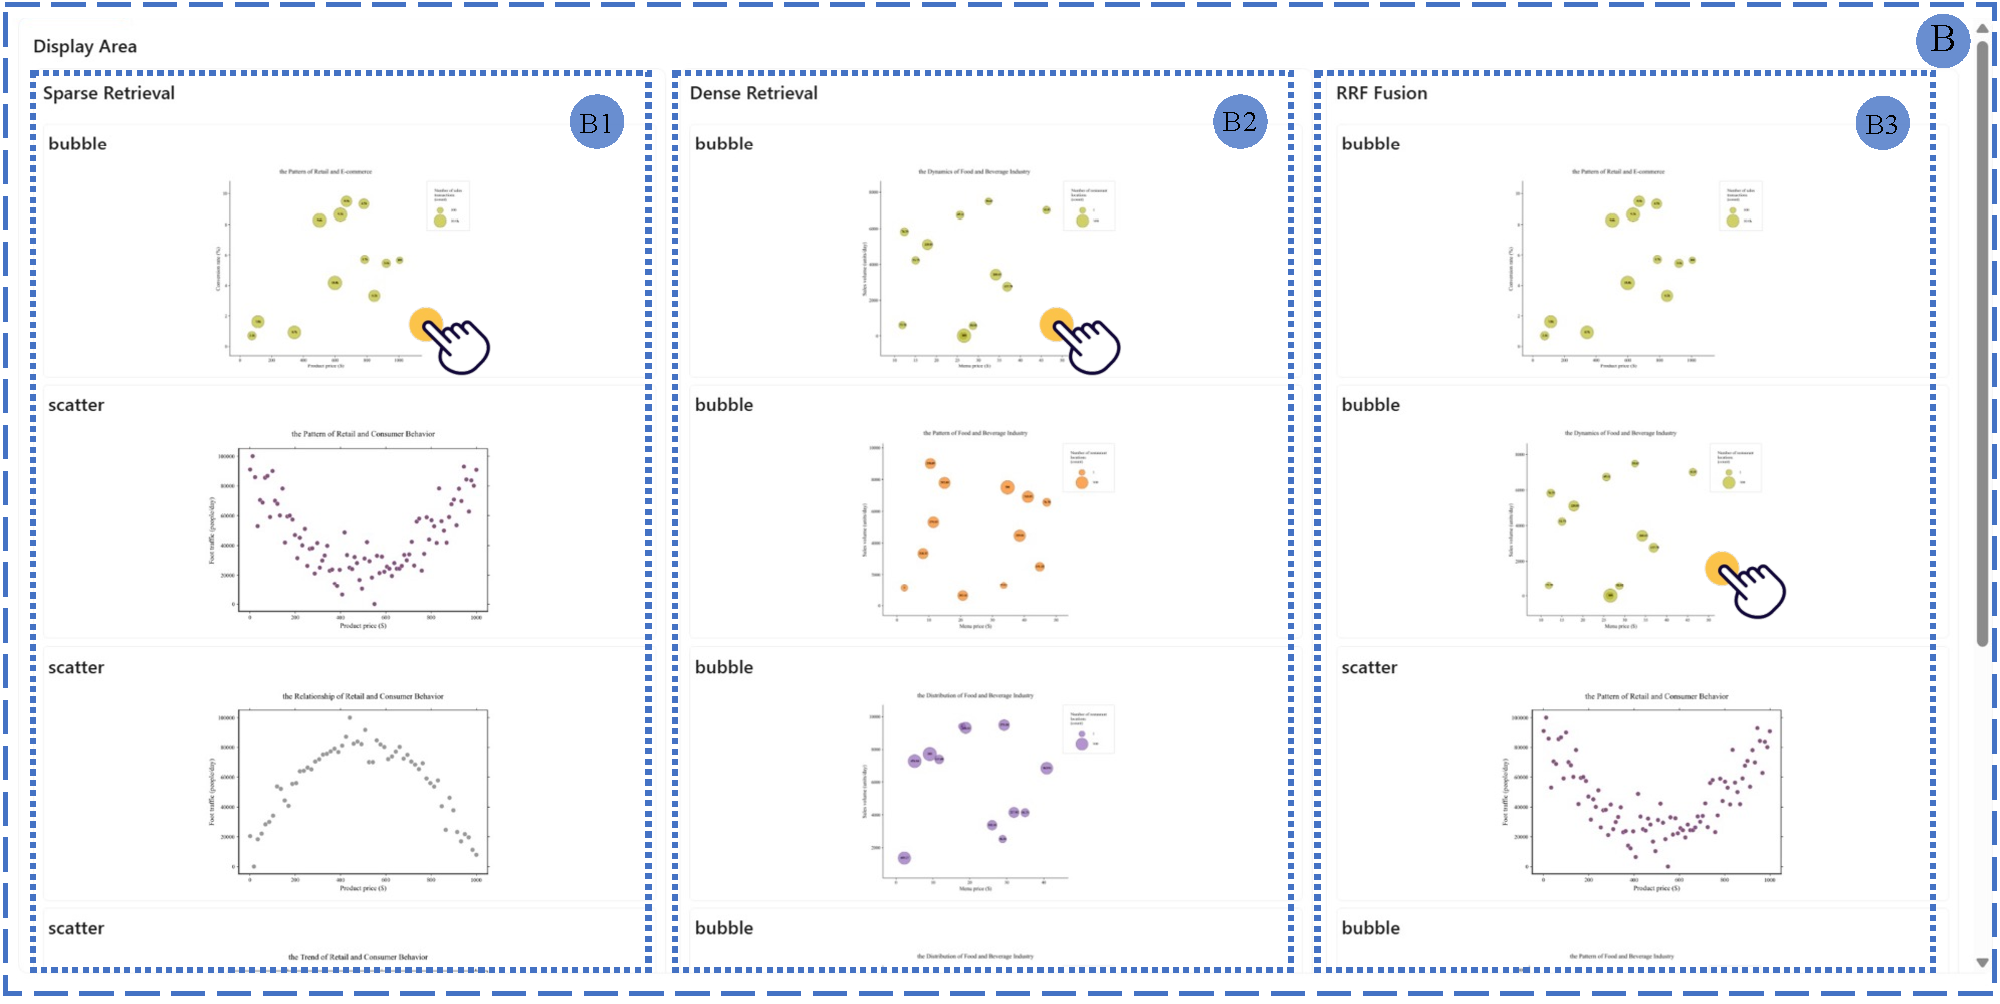
\includegraphics[width=\linewidth]{pics/Display_area.pdf}
    \caption[检索结果展示区]{检索结果展示区\zjutfigcaptionen{Retrieval Result Display Area}}
    \label{fig:display_area}
\end{figure}

\subsubsection{图表推荐准确性}

推荐系统如图\ref{fig:teaser} 所示。用户首先输入想要可视化的文本（A），然后点击“推荐”按钮。检索结果显示在展示区（B），其中（B1）显示稀疏检索结果，（B2）显示稠密检索结果，（B3）显示通过 RRF 算法融合后的推荐结果。

在步骤2中，用户根据自身需求，分别从（B1）、（B2）和（B3）中选择最合适的图表类型。用户选择的图表类型作为系统推荐反馈，用于进一步评估推荐准确性。为了从不同角度衡量三种推荐方法，本文采用平均相关性、平均贡献度（ERR）和准确率三个指标。三者的侧重点不同：平均相关性关注推荐列表整体是否与输入文本相关；ERR 关注合适图表在推荐列表中的排序位置；准确率关注推荐结果是否命中用户最终认可的图表类型。

平均相关性用于衡量推荐列表整体与输入文本语义之间的匹配程度。参与者在比较每种方法给出的 Top 5 推荐结果后，对推荐结果是否适合表达当前文本中的数值关系进行相关性判断，相关性评分被归一化到 $[0,1]$ 区间。设测试文本数量为 $N$，参与者数量为 $P$，推荐方法为 $m$，第 $n$ 个文本由第 $p$ 名参与者给出的相关性评分为 $Rel_{n,p}^{(m)}$，则方法 $m$ 的平均相关性计算为：

\begin{equation}
    AvgRel^{(m)} = \frac{1}{NP}\sum_{n=1}^{N}\sum_{p=1}^{P} Rel_{n,p}^{(m)}
\end{equation}

平均相关性越高，说明该方法返回的候选图表整体越能贴合输入文本的语义和数据关系，但该指标不区分相关图表出现在第1位还是第5位。

平均贡献度使用期望倒数排名（Expected Reciprocal Rank, ERR）计算。ERR 通过衡量用户选择图表与推荐图表之间的匹配情况，并综合考虑推荐序列中的排名信息，为系统提供定量排序评估。ERR 算法的数学表达如下：

\begin{equation}
    ERR = \sum_{i=1}^{K} \frac{1}{i} R_i\prod_{j=1}^{i-1} (1 - R_j)
\end{equation}

其中，$K$ 表示推荐图表数量，本文取 $K=5$。$i$ 表示当前正在评估的图表位置。$R_i$ 表示第 $i$ 个推荐图表是否与用户选择匹配的指示函数；当 $R_i=1$ 时，表示第 $i$ 个推荐图表与用户选择一致；当 $R_i=0$ 时，表示不一致。$\prod_{j=1}^{i-1}(1-R_j)$ 确保在第 $i$ 个推荐图表之前，所有图表均未与用户选择匹配。因此，如果用户认可的图表出现在第1位，则 ERR 取值最高；如果该图表出现在较靠后的位置，则贡献按 $\frac{1}{i}$ 衰减；如果 Top 5 中没有匹配图表，则该轮 ERR 为0。表\ref{tab:err} 中的平均贡献度 $Ave_{ERR}$ 是所有测试文本和参与者对应 ERR 值的平均结果。

准确率用于统计推荐结果是否命中用户最终认可的图表类型。对于每个测试文本，若某种方法给出的 Top 5 推荐列表中包含用户选择的图表类型，则记为命中；否则记为未命中。设命中指示变量为 $Hit_{n,p}^{(m)}$，则方法 $m$ 的准确率为：

\begin{equation}
    Precision^{(m)} = \frac{1}{NP}\sum_{n=1}^{N}\sum_{p=1}^{P} Hit_{n,p}^{(m)}
\end{equation}

准确率反映推荐列表是否覆盖用户需要的图表类型，但不考虑该图表在列表中的具体排名。因此，若两个方法准确率相同，ERR 更高的方法通常代表其排序质量更好。

本文计算稀疏检索、稠密检索和 RRF 融合推荐结果的平均相关性、平均贡献度（ERR）以及准确率，如表\ref{tab:err} 所示。从中可以看出，RRF 在相关性、平均贡献度和准确率上均表现优秀，是最能满足用户需求的推荐方法；稠密检索在平均贡献度和准确率上略低于 RRF；稀疏检索在三个方面仍有提升空间。

\begin{table}[htbp]
\centering
\caption[推荐方法评估结果]{推荐方法评估结果\zjuttabcaptionen{Evaluation Results of Recommendation Methods}}
\label{tab:err}
\begin{tabular}{cccc}
\toprule
推荐方法 & 平均相关性 & 平均贡献度($Ave_{ERR}$) & 准确率 \\
\midrule
稀疏检索 & 0.78 & 0.62 & 80\% \\
稠密检索 & 0.82 & 0.68 & 85\% \\
RRF & 0.84 & 0.72 & 90\% \\
\bottomrule
\end{tabular}
\end{table}

\subsubsection{用户体验评估}

完成实验步骤3后，本文收集了15名参与者的调查问卷，并对收集到的问卷进行统计，结果如图\ref{fig:userstudy} 所示。问卷采用5分制李克特量表，共包含5个问题。关于推荐准确性（Q1），参与者的主观感受与第5.2.1节中的结论一致，约73\%的参与者认为实验过程中 RRF 推荐结果最符合其需求。参与者认为三种推荐方法给出的结果多样性相近（Q2），这可能也与数据集中图表种类数量有限有关。在推荐图表与输入文本相关性方面，几乎所有参与者都认为 RRF 给出的推荐高度相关（Q3）。在系统可用性和整体满意度方面，大部分参与者给出了正面评价（Q4、Q5）。

\begin{figure}[htbp]
    \centering
    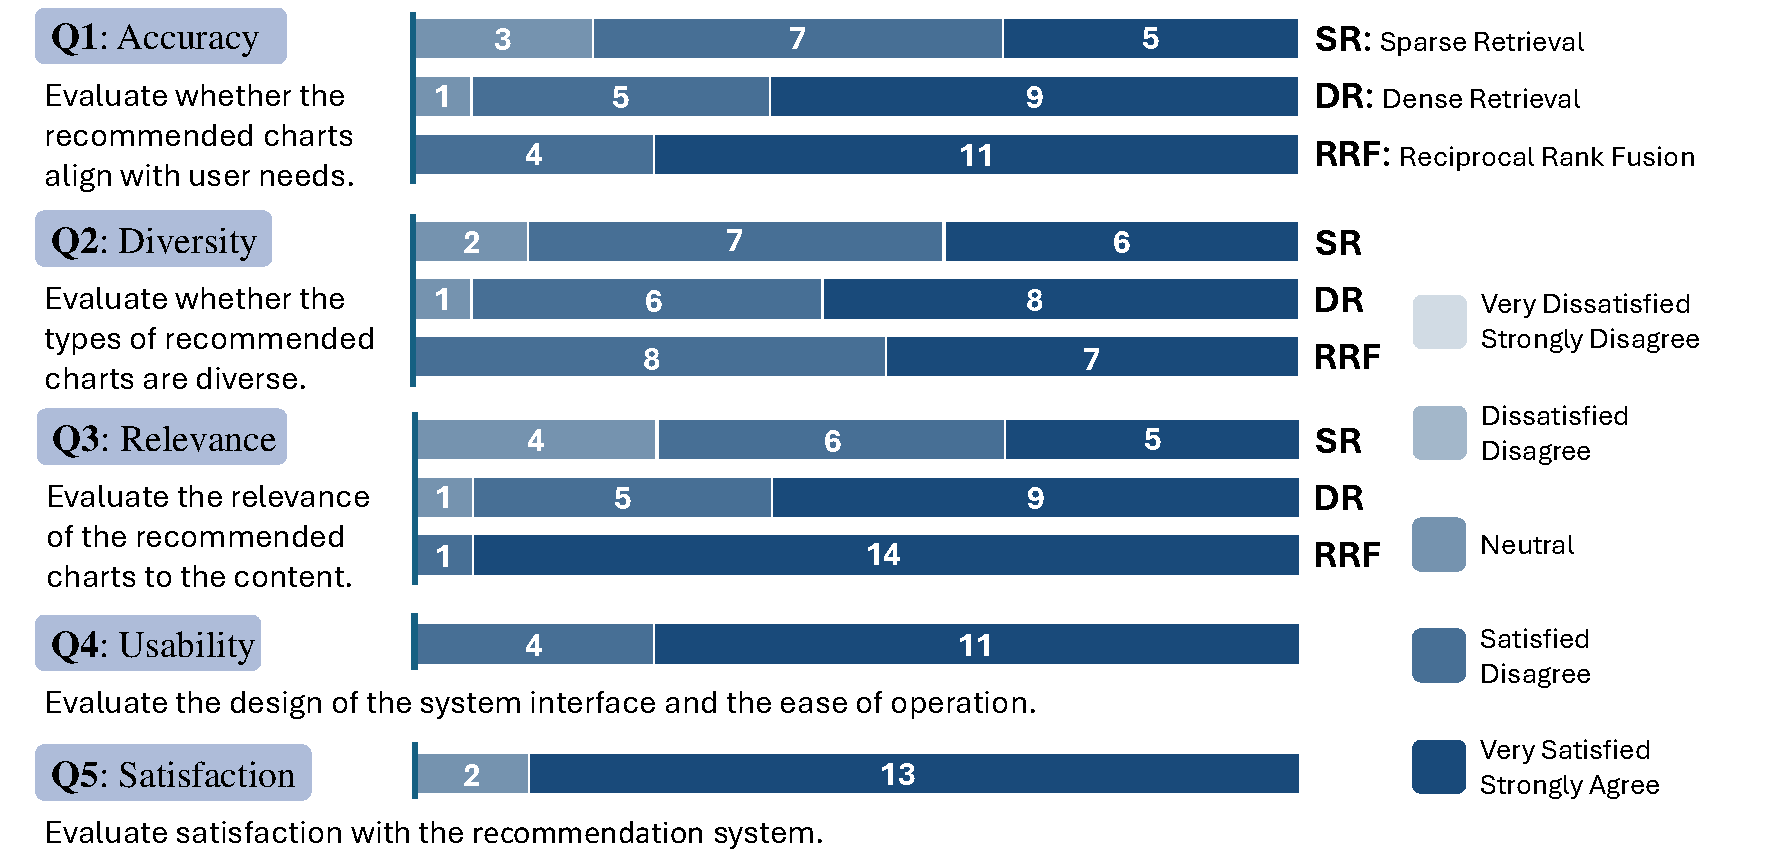
\includegraphics[width=0.8\linewidth]{pics/user_study.png}
    \caption[用户研究问卷结果]{用户研究问卷结果\zjutfigcaptionen{User Study Questionnaire Results}}
    \label{fig:userstudy}
\end{figure}

本文还收集了参与者对推荐系统的开放性反馈，以更好了解其看法和建议。参与者普遍认为该系统使用起来非常方便。用户只需输入文本，系统即可推荐适合体现该文本中数值信息的图表（R1）；三种推荐算法的结果按列排列，也能够帮助数据科学初学者更好理解和解释推荐结果（R2）。参与者喜欢系统编辑区一开始给出初始图表（R5），因为这样不会削弱数据分析的乐趣。他们认为，制图不应完全自动化，因为自动化虽然可以节省体力劳动，但也可能限制创造力。通过算法和系统提供建议，帮助数据分析人员或图表制作者反复迭代和修改（R4），已经能够满足他们的需求和心理预期。

\newpage



